\chapter{Resultados}
\label{chap:resultados}

	Neste capítulo, são apresentadas as avaliações da projeção e da visualização como
	instrumento para avaliação de programas, ambos considerando um conjunto de
	programas escritos em Python para uma disciplina introdutória à Computação. A
	\cref{sec:avalProjecao} e \cref{sec:avalQualitativa} respondem a primeira e
	segunda questão de pesquisa, respectivamente.
	
	
	\section{Descrição da base}
	\label{sec:resultados:base-apoo}

		% TODO: descrição da base
		Essa base é constituída de 152 submissões em Python de 5 problemas distintos.
		Todas elas são oriundas de uma disciplina de programação orientada a objetos
		com a duração de um semestre. No qual, cada aluno é representado por uma
		sequência de números, visto que eles foram anonimizados. Os problemas
		descritos abaixo foram aplicadas por meio de listas de exercícios durante o
		período letivo.
		
		Os problemas tratados foram os seguintes. O primeiro exercício consiste na revisão
		de conceitos básicos como: estruturas de condição e laço de repetição. O segundo
		exercício define a criação de classes com mais de um construtor, e manipulação de
		arquivos e cadeia de caracteres. O terceiro exercício consiste na criação das classes
		\texttt{Palavra} e \texttt{Texto}, no qual a primeira classe deve ser utilizada na segunda
		classe, e uma classe para gerar orações gramaticais. O quarto exercício refere-se a
		utilização de herança e polimorfismo, identificando cada palavra contida em um arquivo. O
		quinto exercício consiste na alteração de uma classe, implementando sobreposição de
		operadores. 
		
	
	\section{Avaliação da projeção com preservação de vizinhança}
	\label{sec:avalProjecao}

		A \foreign{ScienceView} utiliza a preservação da vizinhança
		(\cref{subsubsec:vizinhanca}) para verificar a qualidade das projeções. A \cref{fig:neighborhoodAPOO30}
		apresenta a qualidade da projeção para essa base de dados. Essa técnica visa avaliar
		se houve uma preservação da vizinhança dos objetos no espaço de alta dimensionalidade
		na projeção. A \foreign{Neighborhood Preservation} é calculada tomando os $k$ vizinhos
		mais próximos de uma instância no espaço de alta dimensionalidade e os $k$ vizinhos
		mais próximos na projeção, e verificando-se que proporção da vizinhança é preservada
		na projeção. A precisão final para um dado valor de $k$ é a média das precisões para
		cada instância. Esse cálculo é feito para vários valores de $k$ (tipicamente $k = [1,...,30]$)
		de forma a obtermos uma curva. Quanto mais altos os valores da curva para cada valor
		de $k$, maior a qualidade da projeção. Considerando que a técnica \acl{T-LSP} \cite{Alencar}
		gera uma sequência de projeções, temos uma curva para cada projeção da
		sequência.
		
		% TODO: correção da figura e atualização do parágrafo abaixo
		Por exemplo, na \cref{fig:neighborhoodAPOO30}, na qual cada curva representa um dos cinco
		problemas citados anteriormente, é possível observar que as projeções no início da
		sequência apresentam maior qualidade quando comparada as demais, como é possível observar
		nas curvas dos problemas 3, 4 e 5. Isso é esperado, dado que, além de serem considerados
		mais submissões, as submissões referentes aos problemas 3, 4 e 5 são mais complexos do que
		aqueles referentes aos problemas 1 e 2, com características mais diversificadas e difícil
		representação com precisão no espaço 2D da projeção. 
	
		\begin{figure}
			\centering
			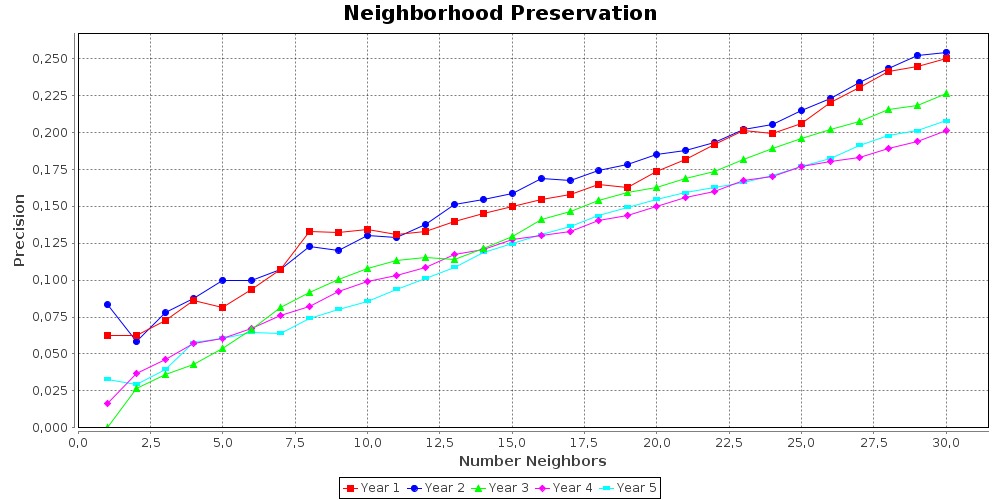
\includegraphics[width=0.85\linewidth]{imagem/neighborhoodAPOO30}
			\caption{Qualidade da projeção, utilizando a preservação de vizinhança (\foreign{neighborhood preservation}).}
			\label{fig:neighborhoodAPOO30}
		\end{figure}	

		% TODO: referência da qualidade da projeção
		Finalmente, observa-se a precisão de 20\% para a linha $5$, obtida com 30 vizinhos
		para a projeção considerando todos os problemas (e, consequentemente, todas as
		submissões). Considerando outros trabalhos que utilizam esta medida para avaliação
		de qualidade de projeções~\cite{phd:paulovich}, a qualidade da projeção é adequada
		e compatível com outras projeções feitas com a técnica LSP e similares, visto
		que obteve resultado semelhante aos obtidos por \citeonline{phd:paulovich}.
	
	\section{Avaliação qualitativa da visualização}
	\label{sec:avalQualitativa}
	
		% TODO: inserção e descrição do fluxograma
		A \cref{fig:fluxogramaEstudo} apresenta os estágios realizados no estudo para
		obter os resultados qualitativos dessa pesquisa. O estudo inicia-se com o
		treinamento, seguido de duas etapas de correções das submissões utilizando a
		ferramenta \foreign{ScienceView} e apenas a tabela de medidas (\cref{apendice:pep8}),
		finalizando com o questionário (\cref{apendice:questionario}). A coluna a direita
		mostra o tempo de duração em minutos de cada etapa, com exceção do questionário
		que os voluntários responderam sem qualquer tipo de contagem de tempo.
		
		\begin{figure}
			\centering
			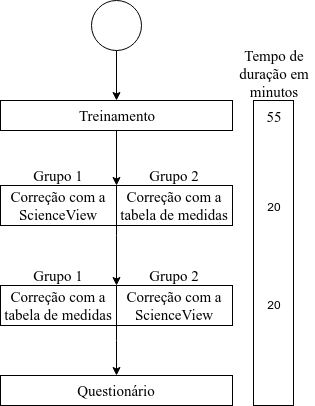
\includegraphics[width=0.4\linewidth]{imagem/fluxogramaEstudo}
			\caption{Fluxograma do estudo da avaliação qualitativa da visualização}
			\label{fig:fluxogramaEstudo}
		\end{figure}
		
		% TODO: descrição do treinamento
		O treinamento foi realizado na forma de tutorial com a apresentação dos critérios
		de avaliação (estilo de escrita e complexidade ciclomática) e da ferramenta com
		duração de $55$ minutos. Especificamente quanto à ferramenta, foram apresentados
		todos os passos referentes ao seu funcionamento, desde a inserção de uma nova
		coleção no banco de dados até a visualização das submissões com a visualização
		da projeção criada a partir da coleção. Em seguida, foi apresentado como utilizar
		a ferramenta para auxiliar na avaliação das implementações: visualizar os
		agrupamentos formados ao longo das projeções, selecionar um determinado conjunto
		de implementações, identificar as características semelhantes de tais grupos e
		abrir mais de uma implementação simultaneamente. Durante o treinamento, foi utilizada uma
		base de dados distinta da descrita na \cref{sec:resultados:base-apoo} para não
		enviesar o estudo.
		
		% TODO: informar que eles tiveram 20 minutos para avaliar trabalhos. 
		Encerrado o treinamento, procedeu-se para correção das submissões com a base
		descrita na \cref{sec:resultados:base-apoo} com duração de $20$ minutos para
		cada uma das duas etapas da correção. Para iniciarmos as correções, foi
		pedido para que os participantes encerrassem o funcionamento da \foreign{ScienceView}
		e a executassem com a criação da base de dados. O estudo teve participação
		de 4 pessoas, devido vossa disponibilidade, e ambos os grupos utilizaram os
		dados obtidos pela \foreign{ScienceView-Python} (\cref{sec:scienceView-Python}).
		Todos os contribuintes realizaram a correção manual, o qual consistiu na correção
		somente do código-fonte, utilizando a tabela de medidas (\cref{apendice:pep8}),
		e somente 3 pessoas utilizaram a ferramenta \foreign{ScienceView} para auxiliar
		na correção. Essa etapa de correção consistiu em duas fases, todas envolvendo a
		correção das submissões, considerando os tipos de erros apontados na extração
		de características e a criação de um relato com os programas avaliados e
		comentários de correção.

		Na primeira etapa da correção, 2 voluntários realizaram a correção manual,
		utilizando a tabela de medidas identificados pela ScienceView-Python, enquanto
		os outros 2 utilizaram a ferramenta ScienceView para auxiliar na correção. Na
		segunda etapa da correção, um dos contribuintes que realizou a correção manual
		passou a utilizar a \foreign{ScienceView}\footnote{O outro participante não
		conseguiu executar a ferramenta ScienceView e não participou desta parte do
		estudo.}, enquanto os 2 que utilizaram a ferramenta na etapa anterior, realizaram
		a correção manual. Os participantes utilizaram a ferramenta sem ajuda no que já
		tinha sido apresentado e o avaliaram por meio de um questionário. 	

		\begin{figure}[b]
			\centering
			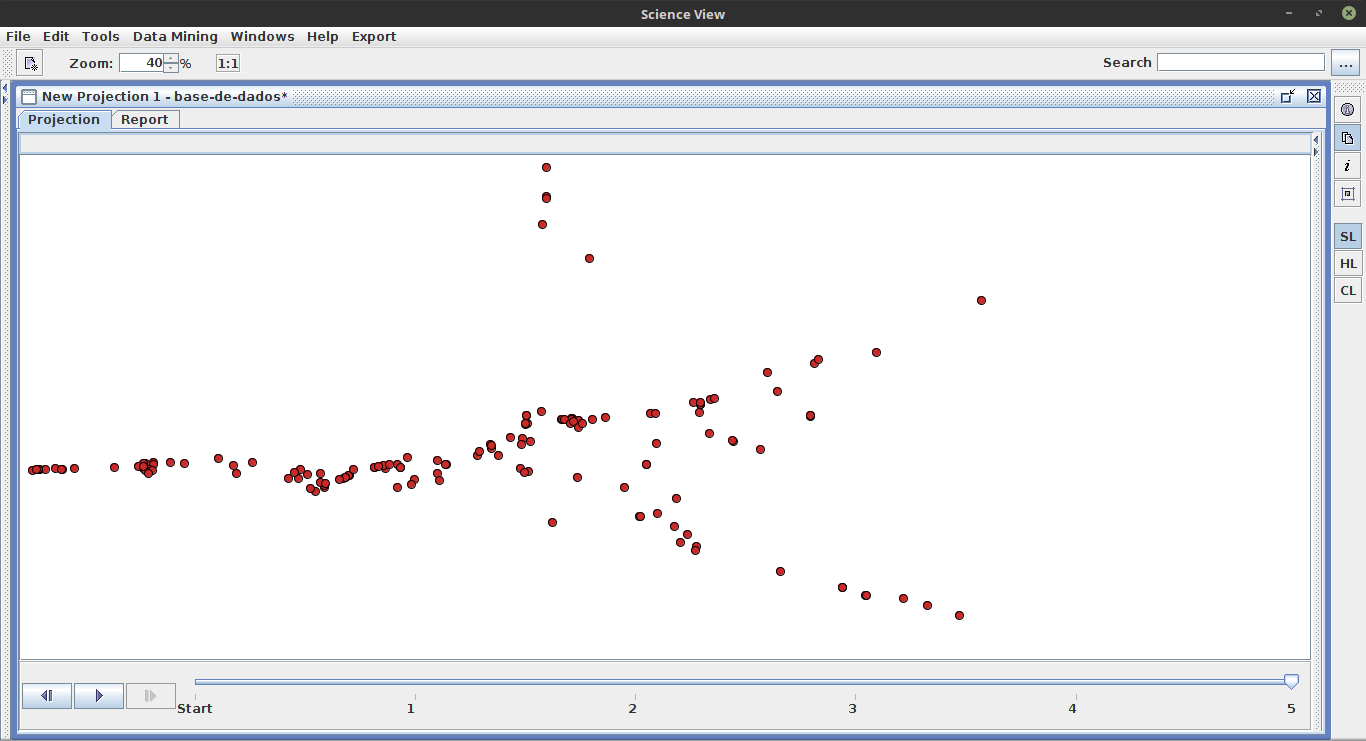
\includegraphics[width=1\linewidth]{imagem/projecaoFinal}
			\caption[Visualização da projeção da base de dados gerado pela \texttt{ScienceView}]
			{Visualização dos agrupamentos da base de dados gerado pela \texttt{ScienceView}.}
			\label{fig:projecaoFinal}
		\end{figure}

		A \cref{fig:projecaoFinal} apresenta a visualização dos agrupamentos das 152
		submissões contidas na base de dados. Isso foi possível após a adaptação da
		ferramenta para leitura de arquivos no formato \texttt{CSV}. Cada ponto da
		visualização é referente a uma submissão. Ao clicar em um dos pontos,
		uma interface exibe sua implementação e as características extraídas pela
		\foreign{ScienceView-Python} para aquela submissão. Também é possível ordenar
		as colunas de características \foreign{Quantity} e \foreign{Normalized} em
		ordem  crescente ou decrescente para visualizar as características que mais
		ocorreram. Por padrão, a tabela é apresentado ordenada de forma decrescente
		pela coluna \foreign{Normalized}.
		
		% TODO: Wiese levantou dúvidas quanto ao "comentário". Substitui por "avaliação" e alterei um pouco o texto
		A \cref{tab:resultados} apresenta a quantidade de implementações que cada
		participante corrigiu e de avaliações realizadas pelo voluntário a fim de
		auxiliar o aluno na aprendizagem. A primeira linha identifica
		qual participante realizou as correções e a primeira coluna indica a forma
		de correção realizada pelos voluntários. Então, é apresentado a quantidade
		de correções que cada participante conseguiu realizar e a quantidade de
		avaliações conforme o tipo de correção.
		
		\begin{table}[h]
			\small
			\begin{tabularx}{\linewidth}{|X|X|X|X|X|}
		        \hline
		        
		        & Voluntário 1 % Bruna
		        & Voluntário 2 % Guilherme
		        & Voluntário 3 % Narci
		        & Voluntário 4\\ % Wagner
		        
		        \hline
		        Correção tradicional
		        & 3 códigos-fontes e 3 avaliações % Bruna
		        & 4 códigos-fontes e 20 avaliações % Guilherme
		        & 3 códigos-fontes e 8 avaliações % Narci
		        & 5 códigos-fontes e 11 avaliações\\ % Wagner
		        
		        \hline
		        \foreign{ScienceView}
		        & Não utilizou a ferramenta % Bruna
		        & 4 códigos-fontes e 4 avaliações % Guilherme
		        & 3 códigos-fontes e observou que a ferramenta auxiliou no encontro dos erros de forma mais rápida. % Narci
		        & 4 códigos-fontes e 8 avaliações\\ % Wagner
		        \hline
			\end{tabularx}
			\caption{Quantidade de correções e avaliações realizados com e sem a utilização da ferramenta}
			\label{tab:resultados}
		\end{table}
		
		Apesar dos 3 voluntários afirmarem que a \foreign{ScienceView} colaborou
		para a correção das implementações, 2 deles corrigiram a mesma quantidade
		de implementações utilizando a ferramenta e manualmente. A exceção ocorreu com 
		apenas 1 participante que extraiu os tópicos semelhantes manualmente. Na
		primeira extração, selecionou apenas 2 códigos-fontes e observou que os
		erros apresentados na tabela de erros eram semelhantes, visto que observou
		a importação de bibliotecas entre funções ao invés de realizá-las no início
		da implementação. Na segunda extração, selecionou 9 códigos-fontes e constatou
		que os erros ocorreram nas implementações e foi compreendido corretamente
		pela ferramenta.


%		As implementações das \cref{fig:codigo1} e \cref{fig:codigo2} foram consideradas
%		semelhantes, devido aos seus respectivos pontos estarem próximos no mapa de
%		projeção. É possível notar que há diversas semelhanças nos tipos das características
%		extraídas e erros que ocorreram pela coluna \foreign{Normalized}, além da quantidade
%		dessas características apresentadas na coluna \foreign{Quantity}.
%		
%		\begin{figure}[h]
%			\centering
%			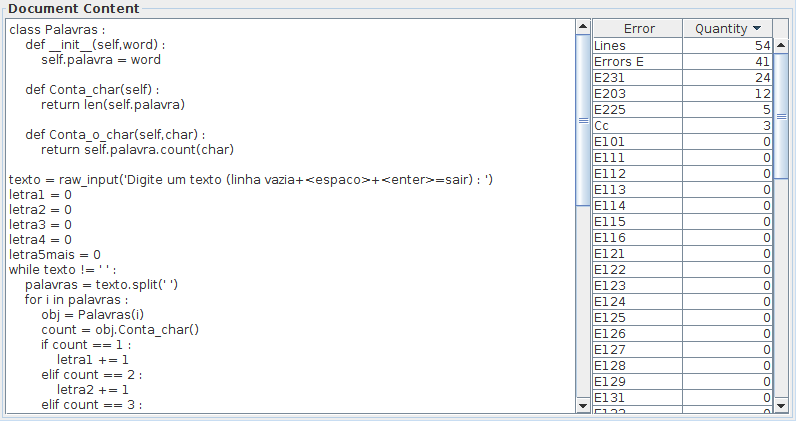
\includegraphics[width=0.8\linewidth]{imagem/codigo1}
%			\caption[Representação parcial da interface que apresenta o código e suas características]
%			{Representação parcial da interface que apresenta o código e suas características \cite{Alencar-etal:2012}}
%			\label{fig:codigo1}
%		\end{figure}
%		
%		\begin{figure}[H]
%			\centering
%			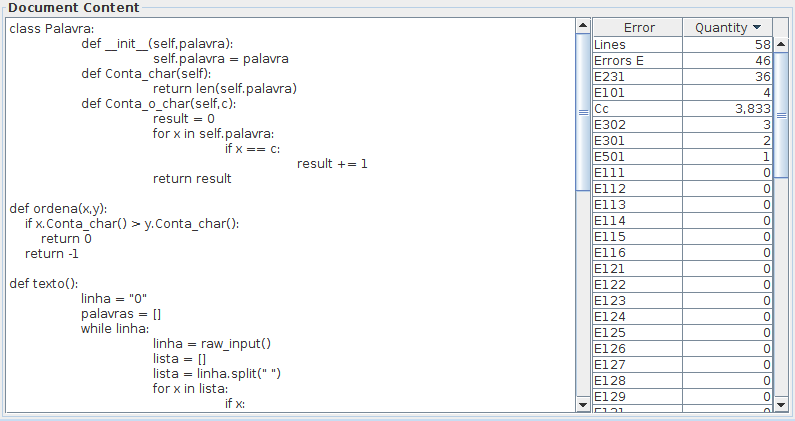
\includegraphics[width=0.8\linewidth]{imagem/codigo2}
%			\caption[Representação parcial da interface que apresenta o código considerado semelhante ao da \cref{fig:codigo1}]
%			{Representação parcial da interface que apresenta o código considerado semelhante ao da \cref{fig:codigo1} \cite{Alencar-etal:2012}}
%			\label{fig:codigo2}
%		\end{figure}
		
	% TODO: criar seção para as respostas do questionário
	\section{Respostas do questionário}
		Para finalizar o estudo, os voluntários responderam um questionário
		anonimamente. O questionário, apresentado no (\cref{apendice:questionario}),
		contém questões objetivas e	dissertativas para sabermos algumas informações
		profissionais do voluntário e avaliar a qualidade do treinamento e da
		ferramenta. Enquanto as questões objetivas visavam as informações profissionais
		e a qualidade do treinamento da ferramenta e se é possível utilizá-la para
		auxiliar na correção, as questões dissertativas visam a encontrar lacunas
		observadas pelo participante para uma possível atualização da ferramenta.
		Um dos participantes não respondeu o questionário.
		
		Sobre o nível de conhecimento em Python, $2$ voluntários afirmaram possuir
		conhecimento intermediário sobre a linguagem de programação, enquanto $1$
		voluntário declarou ter conhecimento básico.		
		
		Acreditávamos que o tempo de experiência como professor poderia interferir
		na quantidade de correções realizadas com a ferramenta, por isso foi questionado
		esse tempo de experiência. Dentre eles, $2$ voluntários possuem menos que $1$
		ano de experiência, enquanto $1$ possui mais de $10$ anos de experiência como
		professor.
		
		Ao serem questionados se o treinamento ajudou a utilizar a ferramenta.
		Todos os respondentes afirmaram que o treinamento em forma de tutorial da
		\foreign{ScienceView} contribui para sua utilização.
		
		Obtivemos êxito com a adaptação da interface que apresenta o código-fonte e a
		tabela de erros, visto que, ao serem questionados se faltava
		alguma informação nessa interface, todos responderam negativamente.
		
		Ao relatarem sobre o \foreign{feedback} recebido da \foreign{ScienceView}
		por meio da visualização da projeção, 2 participantes afirmaram que
		os agrupamentos auxiliaram na verificação de implementações com características
		similares. O outro participantes constatou a possibilidade de utilizar a
		ferramenta em uma turma fechada de alunos a fim de verificar quais os principais
		erros deles por meio da extração de tópicos da ferramenta.
		
		Sobre a experiência em relação ao uso da ferramenta, um dos participantes
		admitiu que, como não utilizou muito a ferramenta, foi mais rápido realizar
		as correções manuais. Contudo, outra resposta afirmou que a utilização mais
		frequente da \foreign{ScienceView}, evidenciará analisar as implementações
		de forma mais rápida.
		
		
% TODO: deixar para artigo
%	
%	\section{Projeção e visualização de MIT 6.00.1x}	
%
%	\subsection{Descrição da base}
%	% TODO: descrever base de dados: quais foram os tipos de programas, quantos foram, falar que a
%	% base não foi anonimizada porque os programas estavam publicamente disponíveis no GitHub.
%	Essa base de dados é constituída de 3470 implementações referente a 10 exercícios
%	distintos. Todos as atividades solicitam manipulação de arquivo e cadeia de caracteres.
%	
%	O primeiro exercício requer conceitos de matriz, utilizando lista dentro
%	de lista, e programação dinâmica para solucionar o transporte de animais.
%	
%	O segundo exercício necessita de conhecimento sobre aleatoriedade, lista, condicional,
%	cadeia de caracteres, operações aritméticas e lógicas para implementar o jogo da
%	forca.
%	
%	O terceiro exercício solicita a utilização de laço de repetição, condicional, lista,
%	operações aritméticas e lógicas para implementar o jogo das palavras.
%	
%	O quarto exercício requer conhecimento de lista e dicionário pra codificar e
%	decodificar um texto.
%	O quinto exercício requer o uso de analisador (\foreign{parser}), construção
%	de classe, interface, polimorfismo e operadores lógicos para desenvolver um programa
%	de monitoramento de novos \foreign{feeds} na Internet.
%	
%	O sexto exercício solicita conhecimento sobre criação de classes, matriz, laço de
%	repetição e manipulação de interface gráfica para implementar um aspirador de pó
%	inteligente e sua simulação.
%	
%	O sétimo exercício consiste no uso de classes, aleatoriedade, laço de repetição,
%	condicional, lista e conhecimento de estatística para implementar uma simulação
%	e um sistema de tratamento de pacientes conforme o vírus que eles possuem.
%	
%	O oitavo problema consiste na implementação de classes a partir do exercício $7$.
%	Pedindo a implementação da classe \texttt{ResistantVirus} e \texttt{SimplePatient}
%	para realizar simulações desses vírus em pacientes.
%	
%	O nono exercício requer o uso de dicionário e operador lógico para desenvolver
%	um software que apresente uma lista de assuntos para cada aluno da universidade.
%	
%	E para o décimo exercício, é necessário conhecer um algoritmo de agrupamento para
%	realizar sua implementação.
%	
%	Os desenvolvedores dessas implementações não foram anonimizados, pois seus
%	códigos-fontes estavam presentes em repositórios públicos no GitHub \cite{github}.
%	
%	% TODO: Marco: colocar a string utilizada para buscar os programas e como foi criada a base
%	
%
%\subsection{Avaliação da projeção com preservação de vizinhança}
%
%
%\subsection{Avaliação qualitativa da visualização}
%% TODO: relatar o estudo: treinamento, instruções, questionário, resultados

	\section{Ameaças à validade}
	\label{sec:ameacas}
	
		O treinamento realizado não foi suficiente para avaliar as implementações por meio
		da utilização da \foreign{ScienceView}, visto que um dos participantes relatou que
		a falta de conhecimento sobre a ferramenta fez com que correção manual acontecesse de
		forma mais rápida. Corrobora com isto a opinião de outro participante, que observou que a ferramenta agilizará
		o processo de correção conforme aumentar a frequência de uso da ferramenta. 
		Principalmente, pudemos observar que os participantes do estudo não consideraram a
		avaliação de grupos de trabalho, optando por avaliar os trabalhos individualmente.
		Dadas essas observações, podemos concluir que o treinamento não foi suficiente para
		capacitar todos os participantes sobre a utilização da ferramenta.
		
		Durante o treinamento, não foi exposto explicitamente que, ao utilizar a \foreign{ScienceView},
		a avaliação é quanto aos códigos-fontes. Com isso, além de corrigirem as implementações,
		alguns participantes buscaram verificar se as características semelhantes apontadas
		pela extração de tópicos realmente ocorriam nas implementações. Isso pode ter
		impactado na correção, devido ao tempo gasto para fazer essas verificações.
		
		Outra ameaça é quanto ao tamanho da base de dados.
		Esta era formada por 152 códigos-fontes que solucionam 5 problemas distintos, algo
		considerado pequeno para um MOOC visto que uma das características do \ac{MOOC} é a grande
		quantidade de usuários (\foreign{massive}). Desta forma, essa base de dados não
		reflete ao montante de submissões que podem ocorrer em um \acs{MOOC}.
		
		Outra limitação é quanto a quantidade de participantes.
		A aplicação do estudo contou com somente $4$ pessoas, e ainda, somente $3$ pessoas
		utilizarem a \foreign{ScienceView}, não nos retorna nada concreto estatisticamente.
		Para
		viabilizar mais participantes, é necessário, além de tempo, a disponibilidade
		de professores para participar do treinamento e utilizar a ferramenta, focando
		que o desenvolvimento do projeto pode contribuir para avaliação de trabalhos,
		além de possibilitar a verificação dos erros mais frequentes a fim de melhorar o
		aprendizado.

	\section{Considerações finais}
	
		Por meio dos resultados obtidos, o próximo capítulo apresenta as conclusões deste trabalho, considerando tanto a análise qualitativa quanto a quantitativa.
